\subsection{Resource Management Architecture}
	Figure~\ref{fig:sys:arch} gives a high level overview of the system architecture.
	We have a single load balancer that distributes the load over the application servers in a greedy way (see Section~\ref{sys:arch:load} for details).
	If the total system load is higher than a certain threshold, the load balancer will rent a new server from Amazon EC2.
	In case the total system load is lower than a certain threshold, the load balancer will free up one of the application servers in order to save resources.

	\begin{figure}[H]
		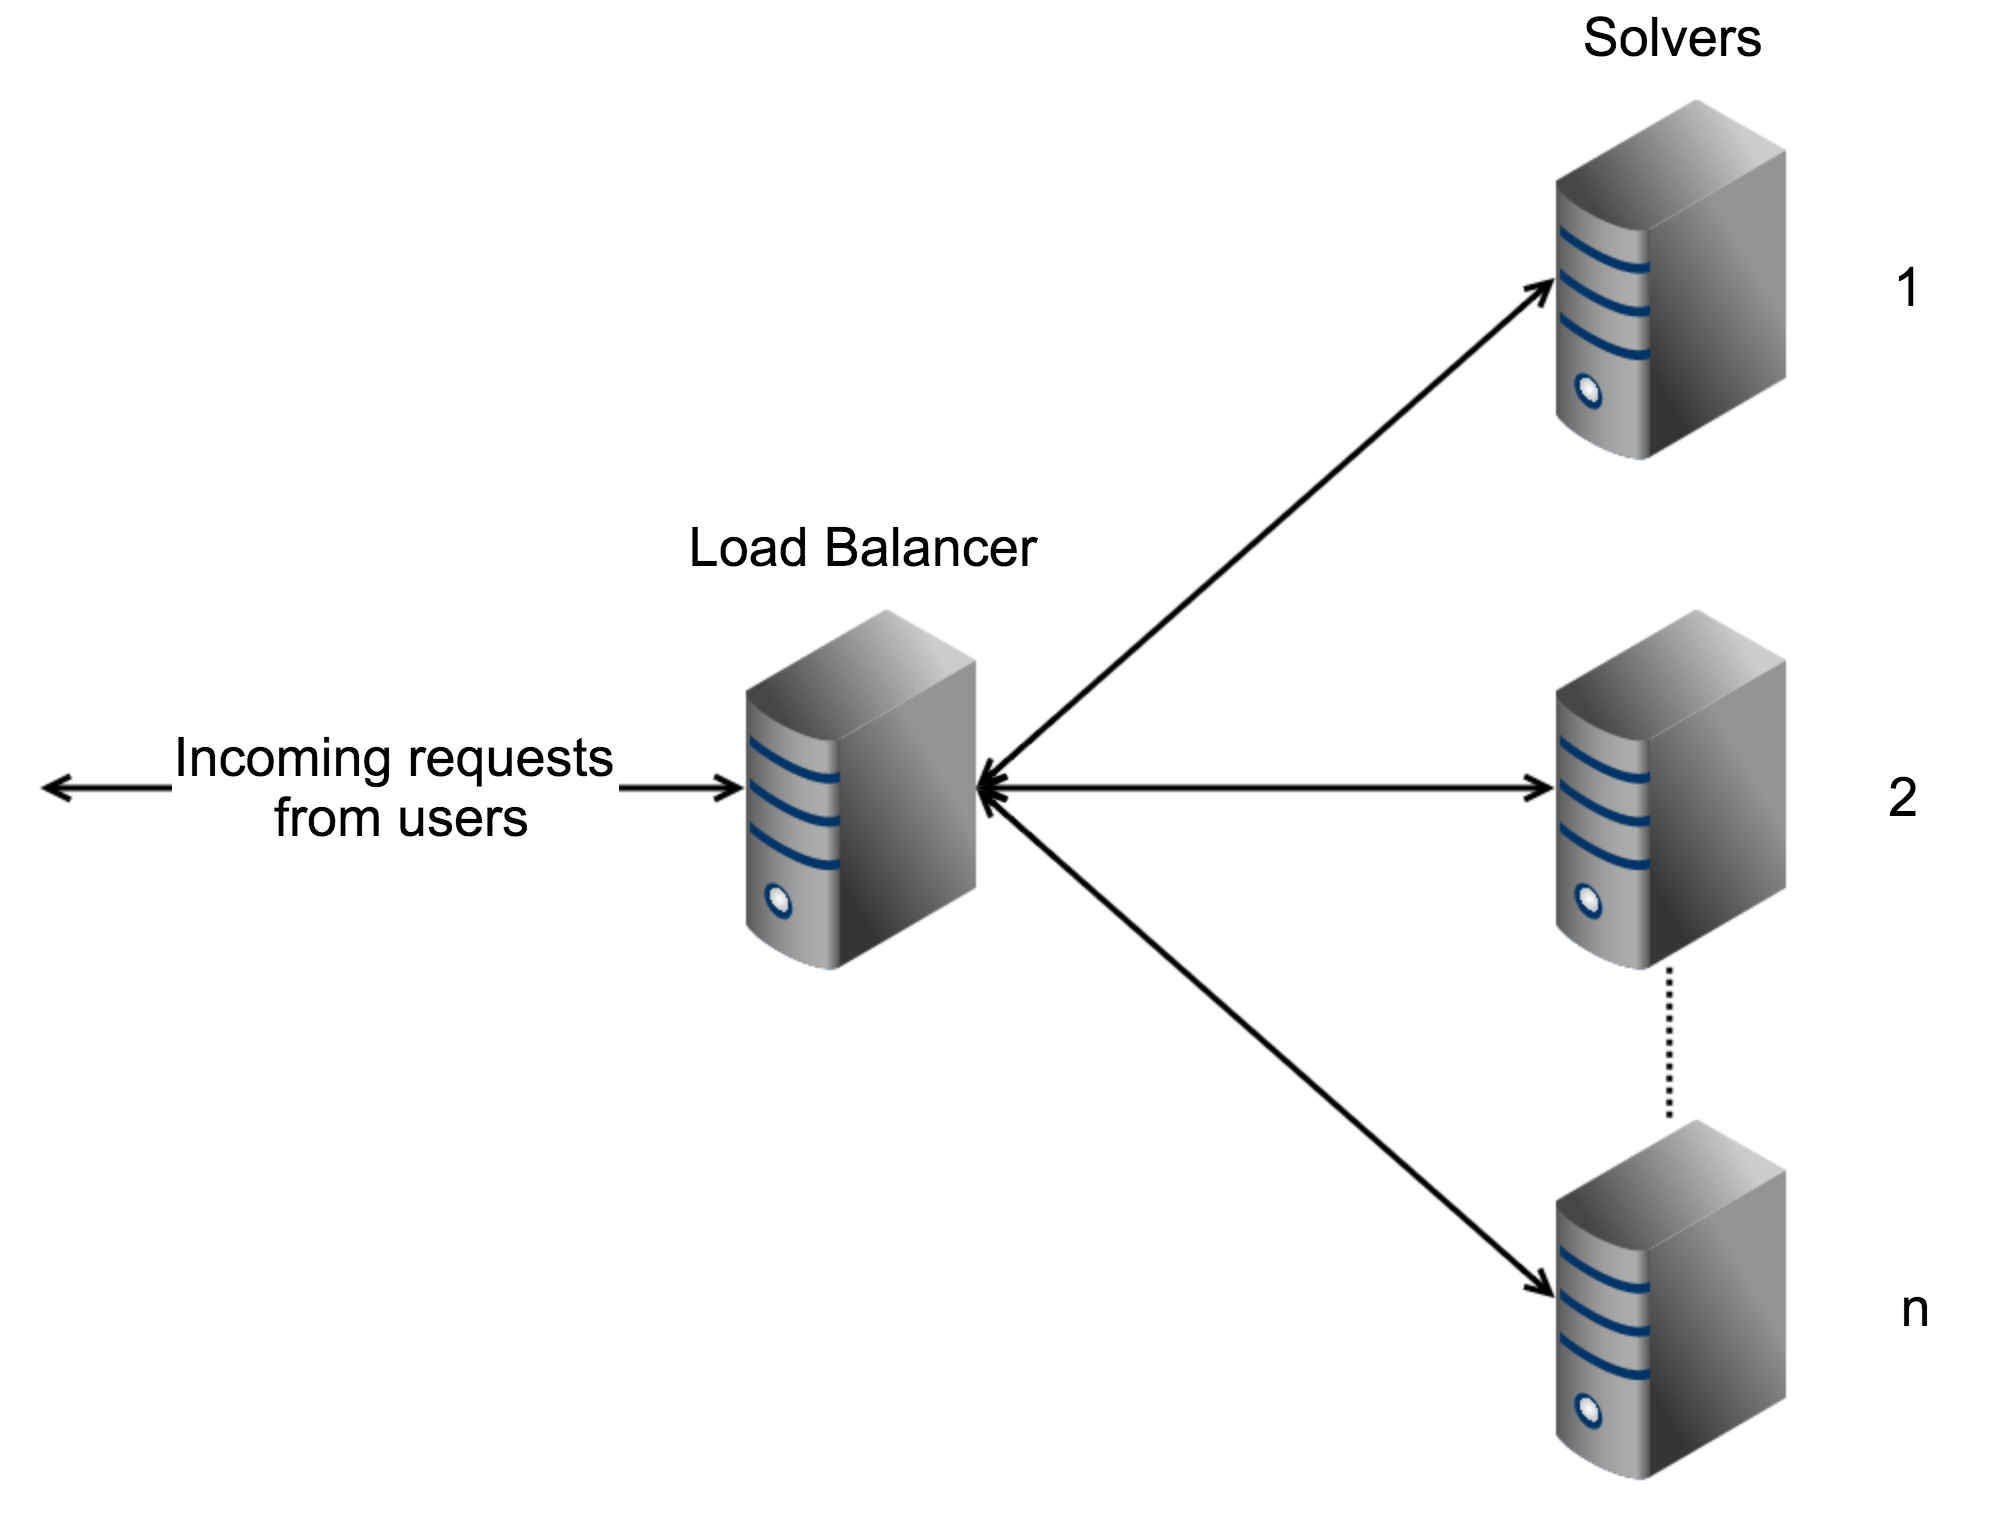
\includegraphics[width=\linewidth]{img/arch}
		\caption{Architecture overview}
		\label{fig:sys:arch}
	\end{figure}

	We will now discuss the system setup.
	Both the application servers and the load balancer use the same basic software stack for their RESTful API interfaces.
	
	We use \textit{nginx} as a web server.
	\textit{nginx} handles all incoming HTTP traffic to the servers, and passes it on to \textit{Phusion Passenger}.
	\textit{Passenger} is an application server that (in our case) will start a \textit{Ruby} process to run our application.
	Within the application, we use the \textit{Sinatra} library to handle HTTP requests.
	
	\subsubsection{Application servers}
		In the application servers, we define the following RESTful endpoint:
		
		\begin{itemize}
			\item \emph{GET:/solution/\texttt{<puzzle>}} Retrieve a completely filled in Sudoku of \texttt{<puzzle>}.
		\end{itemize}

		The API wrapper around the actual application is very simple:
		we first convert the given puzzle to a format that the application can read, then we execute the application with this format and finally we check if the result is valid and if so, return it.

		The application itself is version 0.0.0 of the \textit{sudoku}\footnote{\url{https://rubygems.org/gems/sudoku}} library for Ruby.
		We invoke the backtrack solver on the given puzzle and return the result.
		
		At boot, and each minute, each application server sends a ping message to the load balancer.
		The first time this message arrives, the load balancer registers the application server in the pool.
		The subsequent messages serve as a heart-beat.
	\subsubsection{Load balancer}
		\label{sys:arch:load}

		The load balancer has the following interface:
		\begin{itemize}
			\item \emph{GET:/solution/\texttt{<puzzle>}} Retrieve a completely filled in Sudoku of <puzzle>.
			\item \emph{POST:/ping/\texttt{<instanceid>}} Register a ping message from an application server.
			\item \emph{POST:/cleanup} Do accounting
			\item \emph{GET:/instances} Monitoring, gives a list of all solver machines and their workloads.
			\item \emph{GET:/load} Monitoring, gives an overview of the total system load and the number of active machines.
		\end{itemize}
		
		\paragraph{Balancing}
			The workload size of a request is defined by $1.3^\textnormal{the number of 0-s in the puzzle}$.
			Based on initial tests and knowledge about the application (the use of backtracking), we suspected an exponential relation between the number of zeroes in the request and the processing time.
			However, we were not able to show a good correlation after we ran an experiment with more data.
			See Section~\ref{experiments} for the results of this experiment.
			The constant $1.3$ was found through experimentation and seems to work fairly well.
			
			When the load balancer gets a request, it will forward it to the server with the lowest load.
			Thus, we balance in a greedy way.
			
			If the chosen server does not respond within a time limit, the load balancer will remove it from the pool and retry the request with a different server.
			The end-user does not notice this (aside from the higher-than-normal processing time).
		
		\paragraph{Accounting}
			Every 30 seconds, the cleanup task is run.
			This task removes the workload of each application server by the amount of work a typical application server (all instances are \textit{t1.micro}) can solve in 30 seconds, a parameter to the load balancer.
			
			It also removes application servers that have not sent a heart-beat in 5 minutes from the pool.
			
			Finally, it checks the current server load to see if any new application servers should be started or if any application servers can be terminated.
			We use the following conditions:
			
			\begin{description}
				\item[Start:] $\textnormal{total\_load} > \#\textnormal{instances} * \textnormal{typical\_load} \lor \#\textnormal{instances} < 2$
				\item[Terminate:] $\textnormal{total\_load} < (\#\textnormal{instances} + 1) * \textnormal{typical\_load} \land \#\textnormal{instances} > 2$
			\end{description}
			
			We use the Amazon \textit{aws-sdk} Ruby library to connect to AWS.
			We start an application server by providing the AWS AMI image id for the application server image,
			the instance type (\textit{t1.micro}) and the application server security group (this group is configured to only accept connections from the load balancer).
		
		\paragraph{Monitoring}
			We provide two debugging/monitoring end-points.
			In a production system, these should be protected using some sort of authentication since they give internal information that can potentially be used by an attacker.
			In the current version of our software, the end-points are open to the world.
			
			The \textit{/instances} end-point gives a list of all instances that are currently in the pool.
			For each instance, it reports the Amazon EC2 ID, its IP address, the last time it checked in, and the current load.
			
			We use this to verify that the load balancer actually balances the load properly.
			
			The \textit{/load} end-point gives the number of instances and the current total system load.
			We use this end-point to verify that the system will scale up the number of application server machines under load.

\subsection{System Policies}
	